\chapter{\ifproject%
\ifenglish Project Structure and Methodology\else โครงสร้างและขั้นตอนการทำงาน\fi
\else%
\ifenglish Project Structure\else โครงสร้างของโครงงาน\fi
\fi
}

ในบทนี้จะกล่าวถึงหลักการ และการออกแบบระบบ

\makeatletter

% \renewcommand\section{\@startsection {section}{1}{\z@}%
%                                    {13.5ex \@plus -1ex \@minus -.2ex}%
%                                    {2.3ex \@plus.2ex}%
%                                    {\normalfont\large\bfseries}}

\makeatother
%\vspace{2ex}
% \titleformat{\section}{\normalfont\bfseries}{\thesection}{1em}{}
% \titlespacing*{\section}{0pt}{10ex}{0pt}

\section{ระบบโดยรวมของระบบจำลองการโหวต}
โครงสร้างของระบบจำลองการโหวต ถูกออกแบบเพื่อให้รองรับการโหวตที่ไม่ระบุตัวตน
แต่ยังสามารถยืนยันตัวตนได้ว่าบัตรลงคะแนนเสียงทุกใบ เป็นบัตรที่มาจากผู้มีสิทธิ์ลงคะแนนที่ผ่านการยืนยันตัวตนแล้ว
จึงมีการกำหนดให้มีเซิร์ฟเวอร์สองตัว คอยยืนยันตัวตนผู้มีสิทธิ์โหวต ก่อนจะอนุญาตให้ทำการโหวต โดยมีหลักการทำงานดังนี้
\begin{figure}
\begin{center}
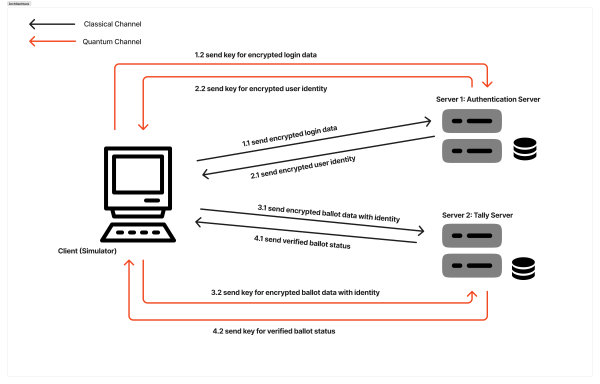
\includegraphics{Auth-Tally2.png}
\end{center}
\caption[Poem]{ภาพรวมและลำดับขั้นตอนของการดำเนินการโหวต}
\label{fig:auth-tally}
\end{figure}

\subsection{เซิร์ฟเวอร์ยืนยันตัวตัน (Authentication Server)}
เซิร์ฟเวอร์ยืนยันตัวตน (Authentication Server) จะเก็บข้อมูลของผู้มีสิทธิ์โหวตทุกคน ว่ามีใครบ้าง และเก็บลักษณะเฉพาะตัว (identity) ของบัตรเลือกทุกใบตั้งไว้ 
ผู้มีสิทธิ์โหวตจะทำการยืนยันตัวตนกับเซิร์ฟเวอร์ยืนยันตัวตนก่อนทำการโหวต โดยการส่งข้อมูลส่วนตัวของตัวเองให้กับเซิร์ฟเวอร์ 
เมื่อเซิร์ฟเวอร์ทำการตรวจสอบและพบว่า ผู้ใช้มีชื่ออยู่ในผู้มีสิทธิ์ จะทำการส่งลักษณะเฉพาะตัว (identity) ของบัตรลงคะแนนกลับไปให้กับผู้มีสิทธิ์โหวต

กระบวนการที่ผู้มีสิทธิ์โหวตส่งข้อมูลส่วนตัวเพื่อรับการยืนยันตัวตน และการที่เซิร์ฟเวอร์ส่งลักษณะเฉพาะตัวของบัตรลงคะแนนกลับมาให้ผู้มีสิทธิ์โหวต 
จะดำเนินการส่งโดยใช้การกระจายคีย์แบบควอนตัม เพื่อรับประกันความปลอดภัยของการส่งข้อมูล

\subsection{เซิร์ฟเวอร์นับและจัดเก็บผลโหวต (Tally Server)}
เซิร์ฟเวอร์นับและจัดเก็บผลโหวต (Tally Server) จะคอยรับบัตรลงคะแนนออนไลน์จากผู้มีสิทธิ์โหวต โดยเซิร์ฟเวอร์ดังกล่าวจะจดจำลักษณะเฉพาะตัวของบัตรลงคะแนนทุกใบได้
ผู้โหวต นอกจากจะต้องแนบผลการตัดสินใจโหวตจะต้องยืนยันตัวตน และทำการแนบลักษณะเฉพาะตัวของบัตรลงคะแนน (identity) มาพร้อมกับผลการโหวตด้วย 
เซิร์ฟเวอร์สำหรับนับและจัดเก็บผลโหวต จะตรวจสอบลักษณะเฉพาะตัวว่าถูกต้องหรือไม่ ถ้าลักษณะเฉพาะตัวไม่ถูกต้อง เซิร์ฟเวอร์จะทำการปฏิเสธบัตรลงคะแนนดังกล่าว
แต่ถ้าลักษณะเฉพาะตัวของบัตรลงคะแนนถูกต้อง จะทำการบันทึกผลการโหวต และทำการระบุว่าลักษณะเฉพาะตัวดังกล่าว ได้ถูกนำไปใช้ในการโหวตแล้ว

เนื่องจากผู้มีสิทธิ์โหวต มีลักษณะเฉพาะตัวของบัตรลงคะแนนไว้กับตัวเอง จึงสามารถเก็บไว้ และสอบถามเซิร์ฟเวอร์นับและจัดเก็บผลโหวตได้ว่า ลักษณะเฉพาะตัวที่ตัวเองเก็บไว้
ได้ถูกใช้ในการโหวตหรือยัง ใช้ในการโหวตตัวเลือกอะไร เพื่อยืนยันความถูกต้องของผลการโหวตได้

กระบวนการส่งข้อมูลการโหวต จะดำเนินการส่งโดยใช้การกระจายคีย์แบบควอนตัม เพื่อรับประกันความปลอดภัยของการส่งข้อมูล


\section{ฟังก์ชันการทำงานของระบบจำลองการโหวต}

ระบบจำลงการโหวตโดยใช้การกระจายคีย์แบบควอนตัม 
ทำการออกแบบให้อยู่ในระบบของ Web Application เพื่อลดความซ้ำซ้อนในการดาวน์โหลดซอฟต์แวร์เพิ่มเติมลงในอุปกรณ์ของผู้ที่สนใจ
และยังทำให้ระบบจำลองเข้าถึงง่ายจากผู้มีส่วนได้ส่วนเสีย ระบบจะมีฟังก์ชันการทำงานทั้งหมดดังนี้



\subsection{ระบบส่งข้อมูลด้วย BB84}
  เป็นฟังก์ชันหลักของระบบจำลองการโหวต โดยจะจำลองการส่งข้อมูลระหว่างผู้มีสิทธิ์โหวต เซิร์ฟเวอร์ยืนยันตัวตน และเซิร์ฟเวอร์นับและจัดเก็บผลโหวต 
โดยใช้ระบบกระจายคียร์แบบควอมตัม และจำลองให้มีผู้ดักฟังคอยตรวจสอบผลการโหวต หลังจากเสร็จสิ้นขั้นตอนการโหวต ระบบจะแสดงผลว่าการจัดส่งข้อมูลด้วยการกระจายคีย์แบบควอนตัม ภายใต้ Protocol BB84 
มีอัตราการตรวจจับการดักฟังสำเร็จในแต่ละขั้นตอน ดังนี้

1. อัตราการตรวจสอบการดักฟังสำเร็จสำหรับขั้นตอนการส่งข้อมูลยืนยันตัวตน 

2. อัตราการตรวจสอบการดักฟังสำเร็จหรับขั้นตอนการส่งเอกลักษณ์ของบัตรลงคะแนน

3. อัตราการตรวจสอบการดักฟังสำเร็จสำหรับขั้นตอนการส่งผลการโหวตไปยังเซิร์ฟเวอร์

\subsection{ระบบยืนยันความถูกต้องของผลการโหวตโดยการใช้เอกลักษณ์ของบัตรลงคะแนน (identity)}
  ระบบจำลองสามารถให้ผู้มีสิทธิ์โหวต ตรวจสอบได้ว่าทำการโหวตอะไรไปกับเซิร์ฟเวอร์ โดยการแนบเอกลักษณ์ของบัตรลงคะแนน
ไปให้กับเซิร์ฟเวอร์ และเซิร์ฟเวอร์นับและจัดเก็บผลโหวต จะทำการส่งผลการโหวตมาให้ผู้มีสิทธิ์โหวต เพื่อเป็นการยืนยันความถูกต้องของสิ่งที่ผู้มีสิทธิ์โหวตได้ทำการเลือก

  ระบบจะแสดงผลการโหวตของผู้มีสิทธิ์โหวตคนดังกล่าว และจำลองการดักฟังข้อมูลในขั้นตอนของการสื่อสารทั้งหมด
และแสดงอัตราการตรวจสอบการดักฟังสำเร็จดังนี้

1. อัตราการตรวจสอบการดักฟังสำเร็จสำหรับขั้นตอนการส่งเอกลักษณ์ของบัตรลงคะแนน

2. อัตราการตรวจสอบการดักฟังสำเร็จสำหรับการส่งผลการโหวตให้กับผู้มีสิทธิ์โหวต

\subsection{ระบบปรับเปลี่ยนความยาวของคีย์ในการเข้ารหัสข้อมูล}
  ระบบจำลอง สามารถให้ผู้ใช้งานระบบจำลอง กำหนดความยาวของคีย์ในการเข้ารหัสข้อมูล โดยสามารถกำหนดได้ตั้งแต่
ความยาว 0.5 เท่าของขนาดข้อความ ไปจนถึง 6 เท่าของขนาดข้อความ เพื่อตรวจสอบว่ากระทบอัตราการตรวจสอบการดักฟังสำเร็จในขั้นตอนต่างๆอย่างไร


\section{โครงสร้างของระบบจำลองการโหวต}
องค์ประกอบทั้งหมดของระบบจำลองการโหวตที่เป็น Web Application สามารถแบ่งได้ดังนี้

\subsection{ส่วนติดต่อผู้ใช้งาน (User Interface)}
เป็นส่วนที่ผู้ใช้งาน สามารถกำหนดค่า และเลือกใช้ฟีเจอร์ต่างๆของระบบจำลองการโหวต

ออกแบบหน้าตาส่วนติดต่อผู้ใช้งานผ่านโปรแกรม Figma และ
พัฒนาโดยใช้โดยใช้ภาษา Typescript บนเฟรมเวิร์ค Vite โดยมีไลบรารีหลักคือ React

\subsection{ส่วนประมวลผลการทำงาน (Server)}
เป็นส่วนที่คอยประมวลผลการทำงานของระบบจำลองผลการโหวต รับการกำหนดค่า และฟังก์ชันการทำงานที่สนใจจากผู้ใช้
แล้วส่งข้อมูลอัตราการตรวจสอบการดักฟังสำเร็จกลับไปหาส่วนติดต่อผู้ใช้งาน

พัฒนาโดยใช้ภาษา Python บนเฟรมเวิร์ค FastAPI สำหรับการส่งข้อมูลไปยังส่วนติดต่อผู้ใช้งาน
มีไลบรารีหลักที่เกี่ยวข้องคือ Qiskit IBM Runtime ขององค์กร IBM Quantum 
สำหรับการเขียนโปรแกรม Quantum Assembly และส่งให้ควอนตัมคอมพิวเตอร์ของ IBM ทำการจำลองการส่งข้อมูลด้วยการกระจายคีย์แบบควอนตัม และส่งผลลัพธ์กลับมาหาส่วนประมวลผลการทำงาน

\subsection{ส่วนฐานข้อมูล (Database)}
เป็นส่วนที่จัดเก็บข้อมูลต่างๆในระบบจำลอง ได้แก้ รายชื่อผู้มีสิทธิ์โหวต รายการของเอกลักษณ์ของบัตรลงคะแนนเสียงแต่ละใบ 
และการกำหนดค่าสำหรับระบบจำลองข้อผู้ใช้แต่ละคน และคอยส่งข้อมูลดังกล่าวให้กับส่วนประมวลผลการทำงาน เมื่อมีการร้องข้อ

เลือกใช้ MongoDB ซึ่งเป็น NoSQL สำหรับการจัดเก็บข้อมูลเนื่องจากสามารถจัดเก็บข้อมูลได้เยอะ มีโครงสร้างการจัดเก็บข้อมูลที่ยืดหยุ่นและปรับได้ตลอดเวลา
ซึ่งเหมาะสำหรับการเก็บรายชื่อผู้มีสิทธิ์โหวต และเอกลักษณ์ของบัตรลงคะแนนแต่ละใบ เนื่องจากมีโครงสร้างที่อาจปรับเปลี่ยนได้ และมีจำนวนข้อมูลมหาศาล

